\documentclass[thesis.tex]{subfiles}

\begin{document}

\chapter{Evaluation}\label{chap:eva}
This chapter will evaluate the proposed algorithms both from a performance and a quality perspective.
In the last section we try to compare our technique to others.
However, as we were not able to implement comparable implementations within the bounds of this project, we can only provide comparisons on an abstract level.

\section{Test Setup and Parameter Overview}
All tests were rendered using a Nvidia GTX670 desktop graphics card.
The test machine has a Intel i7-3770 CPU and uses Windows 8 64bit as OS.

\begin{figure}
\caption{TODO: TEST SCENE OVERVIEW}
\label{fig:testscenes}
\end{figure}
\autoref{fig:testscenes} gives an overview over the test scenes used in this chapter (and throughout the thesis).

How our approach performs depends on several parameters:
\begin{easylist}
\ListProperties(Hide=100, Hang=true, Progressive=4ex, Space=-1.0ex, Space3=-1.3ex, Space*=-1.3ex, Style*=$\bullet\,$,
Style2*=\textbf{--} ,Style3*=$\circ$ ,Style4*=\tiny$\blacksquare$ )
# general
## screen resolution
## number of lights
## reflective shadow map resolution
## number of SH coefficients for diffuse lighting
## number of active caches
### cache address volume resolution
### cascading settings (number, relative size)
### camera (currently visible scene portion)
# shadowing
## shadow lod
## voxel resolution
# specular
## specular environment map resolution
## direct write or cached write
\end{easylist}
The following sections try to give insights on their effects.
We limit our observation to meaningful ranges and do not experiment with arbitrary combinations.

\section{Performance}
In this section the performance and scalability of our approach is examined.
We measure primarily frame times in milliseconds.
To be able to evaluate how specific parts of our algorithm perform, we use OpenGLs timer query functionality to check how long a series of calls take to finish on the GPU (\texttt{GL\_TIME\_ELAPSED}).
The sum of timings from multiple commands may exceed the time a frame takes, since the GPU might work on multiple commands at a time.
However, in our tests this overlap seems to play a minor role since most tasks are either very computational intense or are depending on each other which prohibits parallel command- execution.

\subsection{General Breakdown}
First we want to provide an overview over 

\begin{figure}
\centering
\begin{subfigure}[b]{0.2\textwidth}
\centering
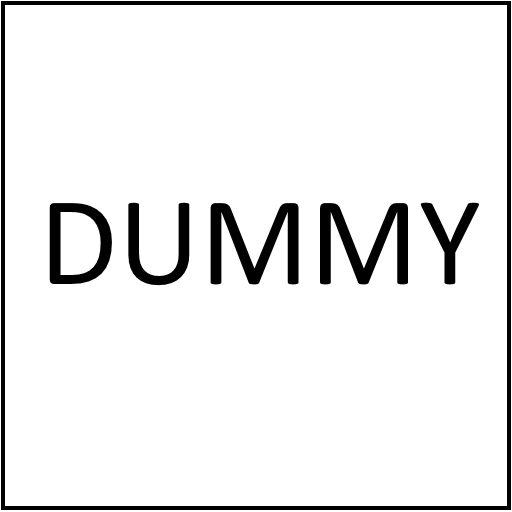
\includegraphics[width=\textwidth]{dummy}
\caption{Scene0}
\end{subfigure}
\\
\begin{subfigure}[b]{0.2\textwidth}
\centering
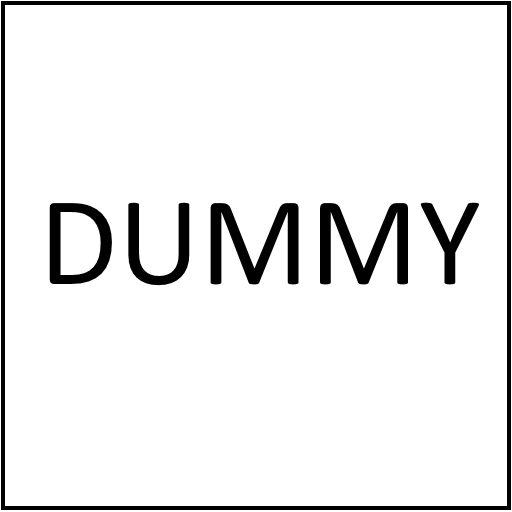
\includegraphics[width=\textwidth]{dummy}
\caption{Scene1}
\end{subfigure}
\\
\begin{subfigure}[b]{0.2\textwidth}
\centering
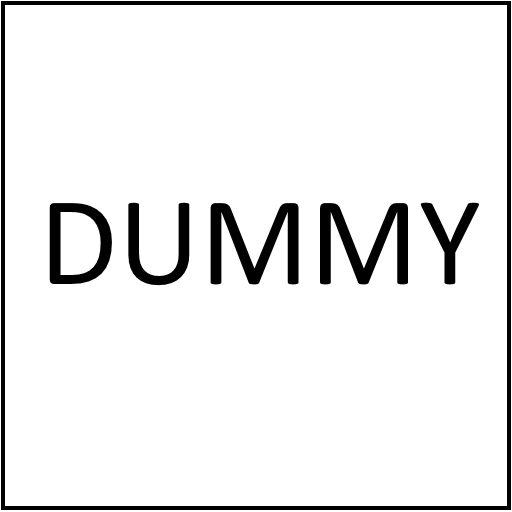
\includegraphics[width=\textwidth]{dummy}
\caption{Scene2}
\end{subfigure}
\caption{Breakdown of frame timings with a moving camera over time for indirect diffuse lighting with shadowing.}
\label{fig:frameratebreakdown:specoff}
\end{figure}
\begin{figure}
\centering
\begin{subfigure}[b]{0.2\textwidth}
\centering
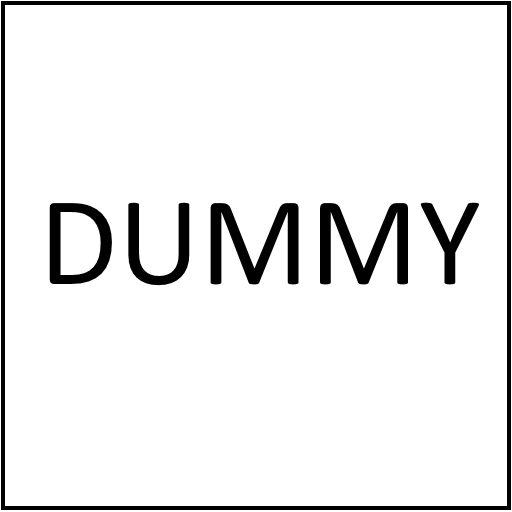
\includegraphics[width=\textwidth]{dummy}
\caption{Scene0}
\end{subfigure}
\\
\begin{subfigure}[b]{0.2\textwidth}
\centering
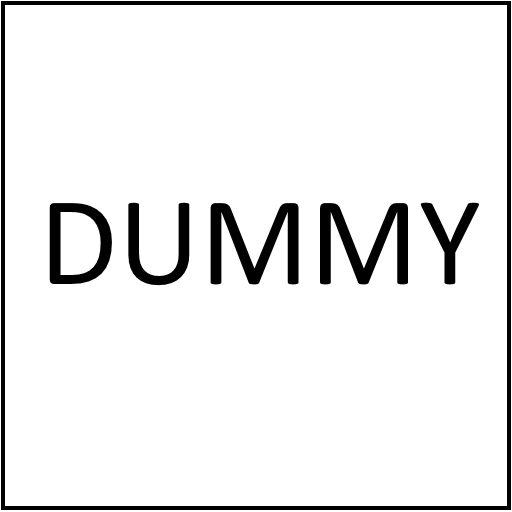
\includegraphics[width=\textwidth]{dummy}
\caption{Scene1}
\end{subfigure}
\\
\begin{subfigure}[b]{0.2\textwidth}
\centering
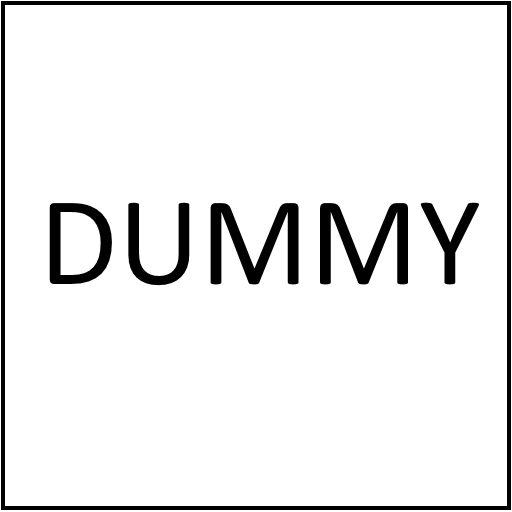
\includegraphics[width=\textwidth]{dummy}
\caption{Scene2}
\end{subfigure}
\caption{Breakdown of frame timings with a moving camera over time for indirect diffuse \& specular lighting with shadowing.}
\label{fig:frameratebreakdown:specon}
\end{figure}

\subsection{Cache Count}
Examine effect of different cachte counts, cascading, CAV, etc.

\subsection{Resolution Dependence}
Examine effect of resolution on prepare and apply passes.

\subsection{Indirect Shadow}


\subsection{Indirect Specular}

\newpage

\section{Quality}
% phenomelogical: "Quality of light, shadow, etc." - which parameters need to be tweaked

\subsection{Sources of Error and Groundtruth Comparision}

\subsection{Artifacts}
regular placement of caches, jaggies,
shadow jaggies,
/interpolation issues

shadow flickering?

\subsection{Temporal Coherency}


\section{Memory Consumption}

\section{Comparison to other Techniques} \label{sec:eva:comparisiontoother}

comparison table, similar to the one in radiance hints?

\subsection{Comparison to LightSkin}

\subfilebib % Makes bibliography available when compiling as subfile
\end{document}